\newpage
\section{Planificació i Gestió del Projecte}

L'objectiu d'aquesta secció és establir un full de ruta clar i realista per al desenvolupament del sistema de votació sobirà en les 14 setmanes disponibles. S'adopta un enfocament de treball iteratiu, que permet encavalcar fases i reduir els riscos d'integració a les setmanes finals.

\subsection{Marc temporal i solapament de fases}

El projecte s'executa entre el 23 de febrer i el 25 de maig de 2026. En lloc d'emprar un model seqüencial estricte (on no es comença una fase fins que acaba l'anterior), s'aplica un solapament estratègic. Per exemple, la interfície web (\textit{Front-end}) es comença a desenvolupar en paral·lel als contractes intel·ligents tan bon punt es defineixen les estructures de dades. Això redueix el camí crític i permet fer proves funcionals molt abans.



\begin{table}[H]
\centering
\renewcommand{\arraystretch}{1.3}
\begin{tabularx}{\textwidth}{|c|l|X|l|}
\hline
\textbf{Setmanes} & \textbf{Fase} & \textbf{Activitats principals} & \textbf{Fita (Milestone)} \\ \hline
1 - 2 & Arquitectura i Entorn & Recerca d'Algorand, definició de la xarxa sobirana i configuració d'AlgorKit. & Entorn local llest \\ \hline
3 - 6 & \textit{Smart Contracts} & Programació del consens (VRF), llista blanca (cens) i ancoratge d'estat. & Contractes testejats \\ \hline
5 - 8 & \textit{Front-end} & Connexió amb Pera Wallet, disseny de la cua cívica i emissió de vots. & Interfície connectada \\ \hline
9 - 11 & Integració i QA & Proves \textit{End-to-End}, resolució de vulnerabilitats i verificació de robustesa. & Beta funcional \\ \hline
12 - 14 & Documentació final & Redacció de la memòria, revisió de codi i preparació de la defensa. & Entrega final (25/05) \\ \hline
\end{tabularx}
\caption{Cronograma de fases iteratives i fites principals}
\end{table}

\subsection{Estimació de l'esforç i distribució de la càrrega}

Per fugir d'estimacions arbitràries, l'esforç s'ha calculat desglossant el projecte en tasques concretes (WBS) i aplicant la tècnica d'estimació de tres punts (PERT) a aquelles àrees on l'equip té menys experiència prèvia, com la programació en la màquina virtual d'Algorand (AVM).

La fórmula emprada per ponderar la incertesa ha estat \( E = \frac{O + 4M + P}{6} \), on \textit{O} és l'escenari optimista, \textit{M} el més probable i \textit{P} el pessimista.

L'esforç total estimat és de \textbf{245 hores}, distribuïdes de manera equitativa per garantir que cap membre pateixi sobrecàrrega i pugui compatibilitzar-ho amb altres assignatures (aproximadament 61 hores per estudiant, a raó d'unes 4,3 hores setmanals).

\begin{table}[H]
\centering
\renewcommand{\arraystretch}{1.3}
\begin{tabularx}{\textwidth}{|l|c|X|}
\hline
\textbf{Àrea de desenvolupament} & \textbf{Hores} & \textbf{Justificació de l'estimació} \\ \hline
\textbf{Gestió i Coordinació} & 35 & Inclou reunions de sincronització setmanals i gestió del repositori. Es calcula a un ritme de 2,5h setmanals compartides. \\ \hline
\textbf{Recerca i Arquitectura} & 40 & Elevada càrrega inicial per entendre la tecnologia VRF, Algorand i dissenyar el concepte de validació via "Nodes efímers". \\ \hline
\textbf{Contractes} & 65 & Estimació PERT aplicada. Inclou la corba d'aprenentatge de Python per a \textit{Smart Contracts} i la lògica criptogràfica de la votació. \\ \hline
\textbf{\textit{Front-end}} & 50 & Estimació per analogia amb projectes previs. Càrrega moderada centrada en React i la integració segura amb la cartera digital. \\ \hline
\textbf{Qualitat i Seguretat} & 55 & Inclou la creació de proves automatitzades per arribar al 80\% de cobertura exigit i la resolució d'errors durant la integració. \\ \hline
\textbf{TOTAL} & \textbf{245 h} & \textbf{\(\sim \) 61 hores / membre} \\ \hline
\end{tabularx}
\caption{Desglossament de l'esforç estimat per àrees}
\end{table}

\newpage
\subsection{Matriu de Responsabilitats (RACI)}

Per garantir una governança àgil, s'ha assignat cada lliurament als rols específics de l'equip. Es defineix qui és responsable d'executar la feina (R), qui n'és l'aprovador final (A), qui ha de ser consultat (C) i qui ha d'estar informat (I).

\begin{table}[H]
\centering
\small
\renewcommand{\arraystretch}{1.3}
\begin{tabularx}{\textwidth}{|X|c|c|c|c|}
\hline
\textbf{Lliurables i Tasques} & \textbf{Coordinador} & \textbf{Arq. i Contractes} & \textbf{Front-end UX} & \textbf{QA i Seguretat} \\
& (Toni) & (Dylan) & (Jordi) & (Marc) \\ \hline
Definició d'Arquitectura i VRF & C & A/R & C & I \\ \hline
Lògica de Contractes (Python) & I & A/R & C & C \\ \hline
Disseny de la "Cua Cívica" i Web & C & C & A/R & C \\ \hline
Proves automatitzades i Auditoria & C & C & I & A/R \\ \hline
Planificació temporal i Riscs & A/R & I & I & C \\ \hline
Integració del sistema complet & C & R & R & A \\ \hline
Redacció de la Memòria Tècnica & A & R & R & R \\ \hline
\end{tabularx}
\caption{Distribució de responsabilitats de l'equip}
\end{table}

\newpage
\subsection{Gestió de riscos Tècnics}

A causa de la naturalesa innovadora del prototip, s'han identificat tres riscos principals i les seves estratègies de mitigació corresponents, dissenyades per no posar en perill l'entrega final:

\begin{itemize}
    \item \textbf{Corba d'aprenentatge d'Algorand:} La programació nativa de la \textit{blockchain} pot endarrerir la Fase 3. \textit{Mitigació:} S'han reservat les primeres dues setmanes exclusivament per a proves de concepte i formació amb la documentació oficial d'AlgorKit.
    \item \textbf{Problemes de sincronització amb \textit{Pera Wallet}:} Les connexions entre dispositius mòbils i aplicacions d'escriptori solen presentar problemes de latència. \textit{Mitigació:} S'iniciarà la integració de la cartera a l'inici de la Fase 4, deixant marge suficient per canviar de llibreria de connexió si fos necessari.
    \item \textbf{Desbordament del camí crític:} Un bloqueig en el codi pot fer saltar la planificació. \textit{Mitigació:} S'ha dissenyat l'arquitectura de forma modular. Si una característica avançada (com l'ancoratge a Ethereum) falla, es pot retallar l'abast i documentar-ho com a treball futur sense invalidar el nucli de la votació.
\end{itemize}

% \section{Planificació inicial del projecte}

% \subsection{Sumari}

% Aquest document estructura la planificació inicial del projecte \textit{Sistema de votació electrònica descentralitzada basat en blockchain}, alineant la gestió del projecte amb les bones pràctiques del \textbf{PMBOK Guide – Eighth Edition}.

% L’objectiu és desenvolupar un prototip funcional descentralitzat, segur, transparent i auditable, amb finalitat formativa orientada a l’aprenentatge de la tecnologia blockchain i els smart contracts.

% El sistema es dissenya per garantir:

% \begin{itemize}
% \item autenticació segura del votant,
% \item emissió d’un únic vot per usuari,
% \item anonimat criptogràfic,
% \item registre immutable dels vots,
% \item verificació pública dels resultats.
% \end{itemize}

% La planificació es basa en principis PMBOK:

% \begin{itemize}
% \item orientació al valor i impacte del projecte,
% \item governança per dominis clau (abast, cronograma, riscos, recursos i stakeholders),
% \item adaptació de pràctiques al context acadèmic i tecnològic.
% \end{itemize}

% El projecte es desenvoluparà durant \textbf{12 setmanes de treball efectiu}, amb entrega final el \textbf{25 de maig de 2026}.

% Els principals artefactes de gestió inclouen:

% \begin{itemize}
% \item Acta de constitució del projecte (Project Charter),
% \item baseline d’abast (enunciat, WBS(EDT) i diccionari WBS(EDT)),
% \item cronograma i fites,
% \item registre de riscos,
% \item matriu RACI,
% \item estimació de costos.
% \end{itemize}


% \subsection{Enfocament de planificació basat en PMBOK}

% La planificació inicial es fonamenta en tres principis:

% \begin{enumerate}
% \item Orientar el projecte al valor: justificar la necessitat i l’impacte.
% \item Governar el projecte per dominis clau: abast, cronograma, riscos, recursos i stakeholders.
% \item Adaptar pràctiques i eines al context acadèmic i tecnològic.
% \end{enumerate}

% La WBS o EDT (Work Breakdown Structure) constitueix l’artefacte base per derivar el cronograma i l’estimació de costos, orientada a lliurables verificables.


% \subsection{Marc temporal del projecte}

% El projecte s’executa entre:

% \begin{itemize}
% \item Inici: 23 de febrer de 2026
% \item Finalització tècnica: 24 de maig de 2026
% \item Entrega final: \textbf{25 de maig de 2026}
% \end{itemize}

% \subsection{Solapament parcial de fases}

% El desenvolupament del projecte es planifica amb un solapament parcial entre fases amb l’objectiu d’optimitzar el temps disponible i reduir els riscos associats a la integració final del sistema.

% En un enfocament seqüencial tradicional, cada fase s’inicia únicament després de finalitzar l’anterior (per exemple: disseny → desenvolupament backend → desenvolupament frontend → integració → proves). Aquest model incrementa la durada total del projecte i concentra els riscos en les fases finals.

% En canvi, el present projecte adopta un enfocament iteratiu i solapat, on determinades activitats s’inicien tan aviat com es disposa de la informació mínima necessària. Això permet avançar en paral·lel sense comprometre la coherència del sistema.

% \subsubsection{Optimització del temps}

% El solapament permet reduir el temps total del projecte. Per exemple, el desenvolupament del frontend pot iniciar-se un cop definides les interfícies de comunicació amb el backend, sense esperar a la finalització completa d’aquest.

% \subsubsection{Reducció de riscos d’integració}

% La integració de components desenvolupats de forma independent és una de les principals fonts de risc en projectes software. El solapament facilita integracions parcials anticipades, permetent detectar incompatibilitats o errors de disseny en fases primerenques, quan el cost de correcció és menor.

% \subsubsection{Validació i retroalimentació primerenca}

% Treballar en paral·lel permet realitzar proves funcionals preliminars abans de la fase final d’integració. Això facilita:

% \begin{itemize}
% \item validar el flux complet de votació,
% \item detectar problemes d’usabilitat,
% \item verificar requisits de seguretat i anonimat,
% \item ajustar decisions tècniques de manera iterativa.
% \end{itemize}

% \subsubsection{Aplicació pràctica al projecte}

% En aquest projecte, el solapament es materialitza de la següent manera:

% \begin{itemize}
% \item el desenvolupament del backend s’inicia mentre es completa el smart contract,
% \item el frontend comença quan les interfícies API estan definides,
% \item les proves s’inicien abans de la integració final,
% \item la validació end-to-end es realitza de forma progressiva.
% \end{itemize}

% Aquest enfocament redueix el camí crític del projecte, millora la detecció precoç d’errors i augmenta la probabilitat d’èxit dins del temps disponible.


% \subsection{Planificació setmanal detallada}

% La planificació setmanal mostra un solapament parcial entre fases. 
% Aquest solapament permet treballar en paral·lel, iniciar el frontend quan les interfícies ja estan definides, validar components abans de la integració final i reduir riscos tècnics. 
% D’aquesta manera es redueix el camí crític del projecte i s’optimitza el temps disponible.

% \begin{table}[H]
% \centering
% \small
% \begin{tabular}{|p{2.5cm}|p{3cm}|p{4.2cm}|p{3.3cm}|p{1.5cm}|}
% \hline
% \textbf{Setmana} & \textbf{Objectiu} & \textbf{Activitats principals} & \textbf{Entregables} & \textbf{Resp.} \\
% \hline
% 1 & Inici formal del projecte & Kick-off, objectius, stakeholders, repositori & Project Charter (borrador) & PM \\
% \hline
% 2 & Baselines inicials & Definició abast, WBS, RACI, riscos inicials & Scope baseline, RACI, riscos v1 & PM + QA \\
% \hline
% 3 & Arquitectura validada & Disseny arquitectura i PoC & Disseny arquitectònic & Backend \\
% \hline
% 4 & Smart contract MVP & Lògica de vot i proves & Smart contract MVP & Backend \\
% \hline
% 5 & Contractei complet & Funcions finals i seguretat & Smart contract v1 & Backend + QA \\
% \hline
% 6 & Backend funcional & API, credencials, integració & Backend MVP & Backend \\
% \hline
% 7 & Frontend votació & UI votació i connexió wallet & Frontend MVP vot & Frontend \\
% \hline
% 8 & Frontend resultats & Resultats públics i millores UX & Frontend v1 & Frontend + QA \\
% \hline
% 9 & Integració total & Integració i proves funcionals & Sistema integrat & QA \\
% \hline
% 10 & Qualitat i seguretat & Tests, revisió logs i correccions & Informe de proves & QA + PM \\
% \hline
% 11 & Documentació & Memòria i presentació & Memòria v0.9 & PM \\
% \hline
% 12 & Tancament & Revisió final i empaquetat & Memòria final i release & Equip \\
% \hline
% \end{tabular}
% \caption{Planificació setmanal del projecte}
% \end{table}



% \subsection{Cronograma del projecte}


% El cronograma del projecte representa visualment la planificació temporal de les activitats principals, mostrant la seqüència de fases, el seu solapament parcial i els punts clau de control fins a l’entrega final.

% Aquesta representació facilita la comprensió del ritme d’execució del projecte, permet identificar dependències entre tasques i evidencia l’optimització del temps mitjançant treball en paral·lel.

% \begin{figure}[H]
% \centering
% 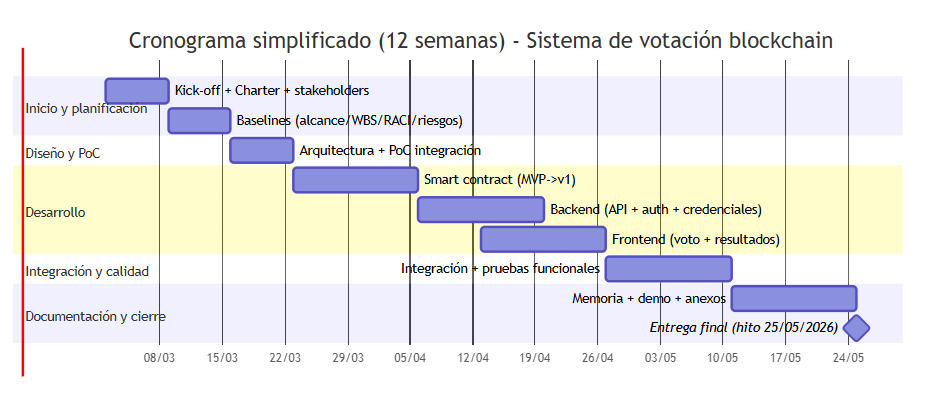
\includegraphics[width=0.95\linewidth]{images/cronograma.png}
% \caption{Cronograma simplificat del projecte}
% \label{fig:cronograma}
% \end{figure}

% \subsection{Fites del projecte}

% Les fites del projecte representen punts clau de control que permeten verificar el progrés, validar els lliurables i assegurar l’alineació amb els objectius establerts. Cada fita marca la finalització d’un resultat verificable i facilita el seguiment del cronograma, la gestió de riscos i la presa de decisions.

% Des d’una perspectiva de gestió de projectes alineada amb PMBOK, les fites constitueixen referències temporals essencials per monitoritzar l’estat del projecte, detectar desviacions i garantir que el desenvolupament avança de manera controlada i coherent amb el pla establert.

% A més, la definició de criteris de verificació per a cada fita assegura que els lliurables siguin objectivament avaluables i que el progrés del projecte pugui ser validat de forma transparent.

% \begin{table}[H]
% \centering
% \begin{tabular}{|p{5cm}|p{3cm}|p{6cm}|}
% \hline
% \textbf{Fita} & \textbf{Data} & \textbf{Criteri de verificació} \\
% \hline
% Project Charter aprovat & 08/03/2026 & Objectius i governança definits \\
% \hline
% Baseline d’abast & 15/03/2026 & WBS i abast validats \\
% \hline
% Arquitectura validada & 22/03/2026 & PoC funcional \\
% \hline
% Smart contract MVP & 29/03/2026 & Tests superats \\
% \hline
% Integració backend & 19/04/2026 & Flux de vot funcional \\
% \hline
% MVP end-to-end & 26/04/2026 & Vot i resultats operatius \\
% \hline
% Beta estable & 10/05/2026 & Proves completes \\
% \hline
% Documentació final & 24/05/2026 & Memòria i annexos complets \\
% \hline
% Entrega final & 25/05/2026 & Lliurament realitzat \\
% \hline
% \end{tabular}
% \caption{Fites principals del projecte}
% \end{table}


% \subsection{Assignació de responsabilitats}
% Per garantir una distribució clara de responsabilitats i una coordinació eficient entre els membres de l’equip, s’ha definit una matriu RACI (\textit{Responsible, Accountable, Consulted, Informed}). Aquesta eina permet identificar de manera precisa qui és responsable de l’execució de cada entregable, qui n’assumeix la responsabilitat final, quins membres han de ser consultats i qui ha de ser informat del seu progrés.

% L’ús de la matriu RACI facilita la comunicació interna, evita duplicitats de tasques i redueix ambigüitats en la presa de decisions. A més, constitueix una pràctica àmpliament utilitzada en la gestió de projectes, ja que contribueix a millorar la governança, la transparència i l’eficiència del treball col·laboratiu.

% En el context d’aquest projecte, la matriu RACI s’aplica als principals lliurables amb l’objectiu d’assegurar una assignació clara de rols i una execució coordinada de les activitats.

% \begin{table}[H]
% \centering
% \small
% \setlength{\tabcolsep}{6pt}
% \renewcommand{\arraystretch}{1.2}
% \begin{tabular}{|p{5cm}|c|c|c|c|}
% \hline
% \textbf{Entregable} & \textbf{PM} & \textbf{Backend} & \textbf{Frontend} & \textbf{QA} \\
% \hline
% Project Charter      & A   & C   & I   & C   \\
% Scope baseline       & A   & R   & R   & C   \\
% Cronograma           & A   & R   & C   & C   \\
% Costos               & A   & R   & C   & C   \\
% Riscos               & A   & C   & C   & R   \\
% Arquitectura         & A   & R   & R   & C   \\
% Smart contract       & C   & A/R & I   & R   \\
% Backend API          & C   & A/R & C   & R   \\
% Frontend             & C   & C   & A/R & R   \\
% Informe proves       & C   & C   & C   & A/R \\
% Memòria final        & A/R & C   & C   & C   \\
% Presentació          & A   & R   & R   & C   \\
% \hline
% \end{tabular}
% \caption{Matriu RACI del projecte}
% \end{table}


% %------------------------------------------------
% \subsection{Diagrama RACI}
% %------------------------------------------------

% El diagrama RACI proporciona una representació visual de la distribució de responsabilitats dins del projecte, complementant la matriu RACI presentada anteriorment. Aquesta representació facilita la comprensió immediata de qui executa cada activitat, qui n’assumeix la responsabilitat final i com es coordinen les tasques fins a l’entrega del sistema.

% El model RACI defineix els rols següents:

% \begin{itemize}
% \item \textbf{Responsible (R):} membre encarregat de l’execució directa de la tasca.
% \item \textbf{Accountable (A):} responsable final del resultat i de la presa de decisions.
% \item \textbf{Consulted (C):} membres que aporten coneixement i suport durant l’activitat.
% \item \textbf{Informed (I):} membres que han de ser informats del progrés o resultats.
% \end{itemize}

% El diagrama mostra el flux de responsabilitats des dels rols tècnics cap als lliurables principals i, finalment, cap a l’entrega del projecte.

% \subsubsection{Anàlisi del flux de responsabilitats}

% El desenvolupament tècnic es distribueix entre els especialistes de cada àrea:

% \begin{itemize}
% \item El \textbf{desenvolupador Back-end + Blockchain} és responsable de la implementació del \textit{smart contract}, component crític que garanteix la seguretat, integritat i immutabilitat del sistema.
% \item El \textbf{desenvolupador Front-end} és responsable de la interfície web i de la interacció amb la blockchain, assegurant una experiència d’usuari clara i funcional.
% \item L’àrea de \textbf{Qualitat (QA)} és responsable de les proves funcionals, la validació del sistema i la generació d’evidències i informes de resultats.
% \end{itemize}

% Aquestes activitats convergeixen en la fase d’integració end-to-end, on es verifica el funcionament complet del sistema.

% \subsubsection{Responsabilitat de governança}

% El \textbf{Project Manager} assumeix la responsabilitat final dels lliurables de planificació i governança, assegurant la coherència entre abast, temps i recursos, així com el compliment dels objectius del projecte.

% \subsubsection{Convergència cap a l’entrega final}

% El diagrama il·lustra com les diferents línies de treball convergeixen cap a dues fites principals:

% \begin{itemize}
% \item la validació tècnica del sistema mitjançant la integració end-to-end,
% \item la verificació funcional i documental a través de les proves i l’informe de qualitat.
% \end{itemize}

% Ambdues línies conflueixen en l’entrega final, garantint que el sistema sigui funcional, verificable i adequadament documentat.

% Aquest enfocament visual facilita la coordinació de l’equip, millora la comunicació interna i assegura una execució ordenada i transparent del projecte.

% \begin{figure}[H]
% \centering
% \begin{tikzpicture}[
% box/.style={rectangle, draw, rounded corners, align=center, minimum width=3cm, minimum height=1cm},
% arrow/.style={->, thick}
% ]

% % Roles
% \node[box] (pm) {Project\\Manager};
% \node[box, below=1.8cm of pm] (backend) {Backend +\\Blockchain};
% \node[box, below=1.8cm of backend] (frontend) {Front-end};
% \node[box, below=1.8cm of frontend] (qa) {QA};

% % Deliverables
% \node[box, right=3.5cm of pm] (planning) {Planificació\\i Governança};
% \node[box, below=3cm of planning] (integration) {Integració\\End-to-End};
% \node[box, right=3.5cm of qa] (testing) {Proves i\\Validació};
% \node[box, right=3cm of integration] (delivery) {Entrega\\Final};

% % Arrows
% \draw[arrow] (backend) -- (integration);
% \draw[arrow] (frontend) -- (integration);
% \draw[arrow] (qa) -- (testing);
% \draw[arrow] (integration) -- (delivery);
% \draw[arrow] (testing) -- (delivery);
% \draw[arrow] (pm) -- (planning);
% \draw[arrow] (planning) -- (delivery);

% \end{tikzpicture}
% \caption{Diagrama RACI simplificat del flux de responsabilitats}
% \end{figure}

% \subsection{Camí crític i dependències}

% El camí crític representa la seqüència d’activitats que determina la durada total del projecte. Aquestes tasques no disposen de marge temporal i qualsevol retard en la seva execució pot afectar directament la data final d’entrega.

% En aquest projecte, el camí crític està format per:

% \begin{itemize}
% \item el desenvolupament del \textit{smart contract}, nucli funcional que garanteix la integritat i seguretat del sistema,
% \item la integració amb el backend, necessària per gestionar credencials i executar el flux de vot,
% \item la integració amb el frontend, que permet la interacció de l’usuari amb el sistema,
% \item les proves end-to-end, imprescindibles per verificar el funcionament complet de la solució.
% \end{itemize}

% Aquestes activitats constitueixen la columna vertebral del projecte i requereixen un seguiment prioritari per evitar desviacions en el calendari.

% \subsection{Gestió de reserves i incertesa}

% En la planificació del projecte s’ha previst una reserva temporal durant l’última setmana, amb l’objectiu de gestionar possibles imprevistos i reduir el risc associat a la fase final d’integració.

% Aquesta reserva permet abordar:

% \begin{itemize}
% \item incidències tècniques inesperades,
% \item ajustos derivats de la integració final,
% \item millores d’usabilitat i estabilitat,
% \item revisió i millora de la qualitat de la documentació.
% \end{itemize}

% La incorporació d’aquest buffer temporal constitueix una pràctica habitual en la gestió de projectes, ja que permet absorbir la incertesa inherent als sistemes tecnològics i augmenta la probabilitat d’assolir els objectius dins del termini establert.